\documentclass[10pt]{report}
\usepackage{listings}
\usepackage{graphicx}
\usepackage{url}

% global commands

\newcommand{\javalst}[2]{
  \lstset{language=Java,captionpos=b,tabsize=4,frame=single,numbers=left,
    numberstyle=\tiny,numbersep=10pt,breaklines=true,showstringspaces=false,
    basicstyle=\footnotesize,emph={label}, caption={#1}, label={#2}}
}
\newcommand{\initlisting}[2]{
  \lstset{language={#1},captionpos=b,tabsize=4,frame=single,numbers=left,
    numberstyle=\tiny,numbersep=10pt,breaklines=true,showstringspaces=false,
    basicstyle=\footnotesize,emph={label}, caption={#2}}
}

\newcommand{\nm}{{\bf proTrade}}
\newcommand{\nmsp}{{\nm \ }}
% end commands
\setlength{\parskip}{0.3cm}
\setlength{\parindent}{0cm}

\begin{document}

\title{\nmsp - A Professional Tennis Trading Environment}

\author{Corina Ciobanu \and Iskander Orazbekov \and Sahin Mir \and Paul Grigoras \and Radu Baltean-Lugojan}

\date{\today}         % inserts today's date

\maketitle            % generates the title from the data above

\begin{abstract}
Tennis trading is a steadily growing market on the Betfair Exchange, with more than 70\% of bets being placed in-play. In order to maintain market liquidity, exchanges must attract customers for example, by supplying them with better tools. By providing more information and better visualization techniques such a tool can help the trader improve his understanding and predict the market evolution, which should (potentially) lead to an increased profit.

In the case of tennis trading, the information required to understand and predict the evolution of the market associated with a particular match consists of the live score, player statistics, potentially a live video feed and - of course - the market data (evolution of betting odds). Ideally, this information is desired for both historical and live matches.

At the moment, no application provides the entire information. A number of solutions exist which allow visualization of historical market data, but they generally lack the more specific, tennis related data. For example the Fracsoft Data Viewer (\cite{site-fracsoft}) does not correlate market data with match data (scores, player statistics). BetAngel (\cite{site-betangel}) provides some tennis related data and prediction, but relies on the user to input the current match score by pushing buttons. This not entirely suited for the high rate with which data is updated. Ideally all the information should be automatically provided to the user to increase update speed and enhance usability.

\nmsp means to fill this gap, by providing all the information, betting and prediction functionalities for both historical and live matches, in an entirely automated fashion.

\end{abstract}

\tableofcontents

\chapter{Introduction}

\section{Importance of Tennis Trading}

This section explains why tennis trading is important, providing background information on the game itself but also on betting and trading.

\subsection{The Game of Tennis }

Tennis is a popular sport played between two players (singles) or between pairs
(doubles). The aim is to win enough points to win a game, enough games to win
a set and enough sets to win a match. Matches are usually played as best of three
sets, but best of five sets are also played in high profile mens tournaments (Grand
Slams). The complex scoring rules lead to a significant number of points being
played in evenly matched games. See Appendix A for the explanation of the Tennis Rules\\
An average tennis match lasts between one and two hours and the average num-
ber of points played is about 150. However, late stage matches of a Grand Slam
tournament often last as much as 4-5 hours and many more points are played.


\subsection{Tennis betting}

Tennis betting is the activity of wagering money on a tennis match with the intention of winning additional money.
The pay out on a winning bet is equivalent to the amount bet multiplied by a coefficient called "odds" set by a bookmaker or a 
counterparty.
Tennis betting is largely popular since tournaments are played all around the year
with huge markets being created around every single match, which represents a
major opportunity for profit. It is possible to place bets both before or during
a match (in-play betting). The unpredictable flow of a tennis match makes in-
play betting very exciting as every single point played leads to a change in odds,
especially during the crucial moments of a match where big changes in odds can be
observed. The volatility of odds observed during a tennis match is very similar to
the stock markets, but over a much shorter period of time.
See Appendix B for a brief introduction to betting\\


\subsection{Tennis Trading}

Tennis is an ideal trading sport due to the large number of points played and the volatility of odds created
by the unpredictable flow of a tennis match. Professional betters can speculate the large
fluctuation of the betting odds during the matches to obtain profit, regardless of
the match outcome. This is known as tennis trading. See Appendix B for a brief overview of tennis trading and an example of trading\\
The following graph represents the trend in the market volume of the tennis betting.

\begin{figure}[ht]
\centering
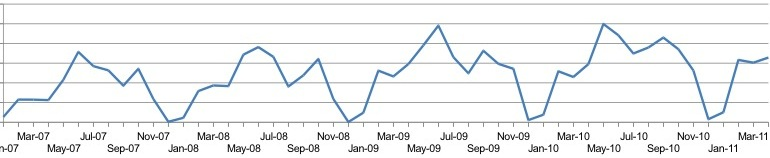
\includegraphics[scale=0.4]{bftennis.jpg}
\caption{}
\end{figure}
\url {http://www.fracsoft.com/index.php?option=com_content&task=view&id=109&Itemid=137}

From the graph above we can clearly observe that the market volume is steadiliy increasing year by year and it's peaking at 
Grand Slams tournaments which are the most important tennis events of the year in terms of public attention, ranking points and prize-money awards.
For example, the market created around the US Open Final 2011 had a value of \pounds40 millions which represents the total value of the bets actually matched.
From the total amount of the matched bets, 70 percent are made in-play, meaning that most of the betters are following the odds trend closely for 
speculative purposes. 
There are several factors which have contributed to the increasing popularity of the tennis trading such as:
\begin{itemize}
\item increasing popularity of the game of tennis 
\item increasing worldwide internet access and a faster internet speed  
\item increasing number of tennis trading platforms
\end{itemize}


\section{State of the Art Applications for Tennis Trading}

Tennis trading is a rapidly developing market, so it is not surprising that there are already quite a few solutions 
that are attempting to fill this niche. However, most of them approach the subject from a too general perspective. 
In order to provide a better overall picture here is the outline.

\subsection{Betfair}

Betfair's own application attempts to cover the whole variety of sports, therefore, losing sharpness in perception 
of the most important events in the tennis world. This in turn leads to an unfriendly user interface, overloaded with 
features that are probably not going to be used in tennis trading environment. Most importantly, the application lacks 
visual features that provide a better picture of the game flow, such as graph chart of odds.

\begin{figure}[h]
\begin{center}
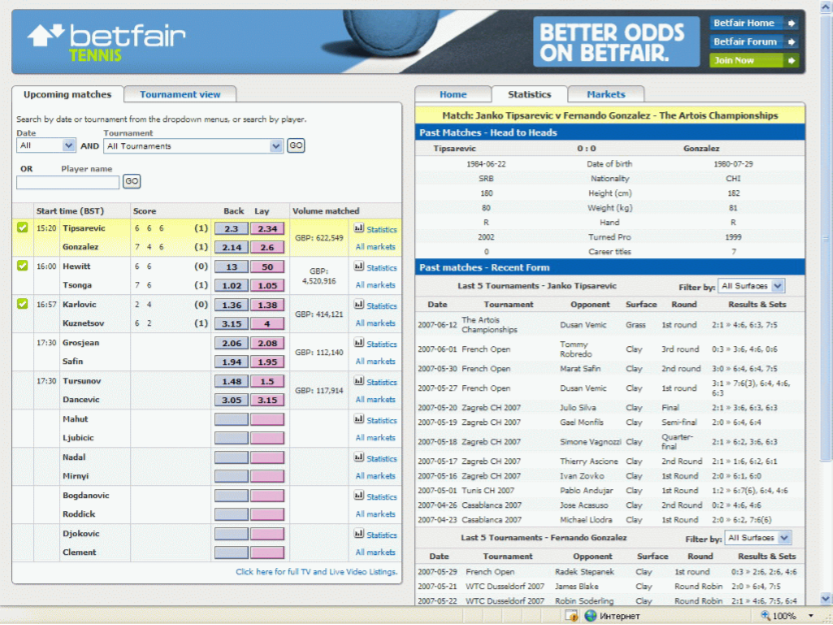
\includegraphics[scale = 0.36]{betfair.png}
\end{center}
\caption{Betfair platform}
\end{figure}

This results in users having not enough information to build their assumptions upon, thus, making it unclear to the 
common trader and, consequently, less attractive than competitors' products on the market.

However, at the same time Betfair's attempt gives a good harness to be used in the project, considering the range of 
features implemented. For example, player statistics provides good background knowledge about the match, whilst latest 
odds give a picture of the actual game.

\subsection{BetAngel}

BetAngel software is also wide in scope of different sports covered, moreover, its particular platforms are more specialised 
in the sport given. Tennis Trader is a very informative application, which, however, does not have many visual features. 
Consequently, it cannot provide a thorough view of the game, leaving out the data that could be given to the end users for 
technical analysis of the market.

\begin{figure}[h]
\begin{center}
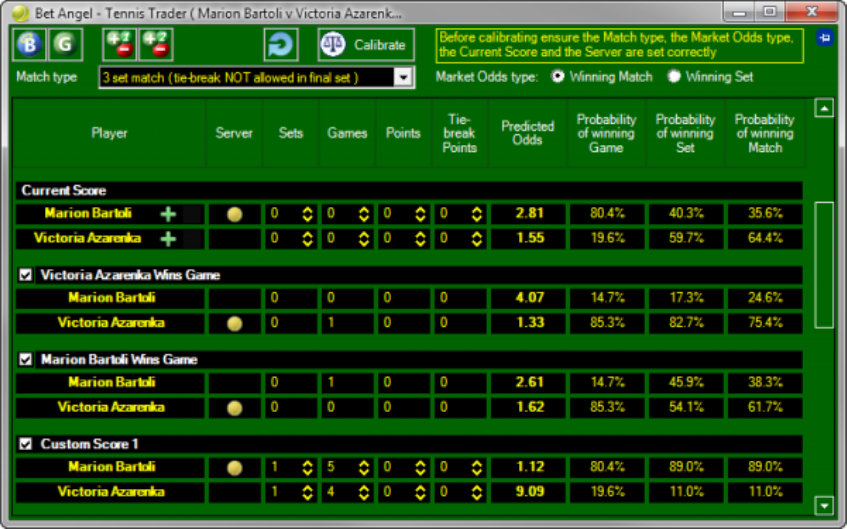
\includegraphics[scale = 0.36]{betangel.png}
\end{center}
\caption{BetAngel Tennis Trader}
\end{figure}

In particular, even though the application provides implied probabilities for different ways the match can take, it does not give 
any previous or background information upon the match, making users rely on the engine provided by the platform. 

\subsection{Fracsoft}

Fracsoft solution is an informative, well-structured platform, that not only provides match figures to the end users, but also gives a better 
picture of the game itself, by drawing out the odds history for the players. However, even though visual part of the application is 
present, some of crucial data is still missing - for example, player statistics that provide background information or implied odds 
engine which is used for own bets correction.

\begin{figure}[h]
\begin{center}
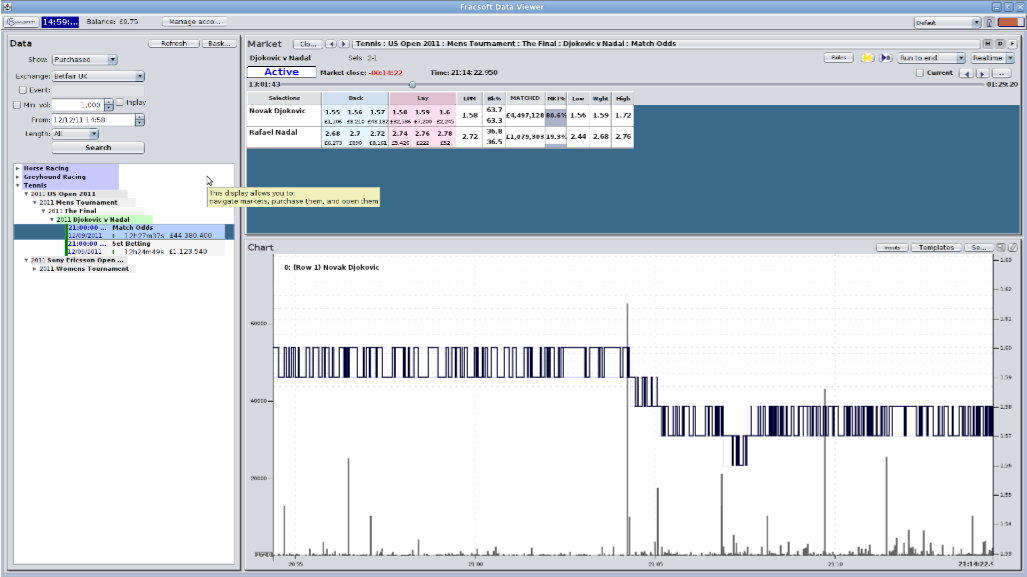
\includegraphics[scale = 0.36]{fracsoft.png}
\end{center}
\caption{FracSoft platform}
\end{figure}

Among many features that were implemented in the FracSoft software there are some that might be unnecessary for the common user, therefore 
overcomplicating the interface. In particular, the relative size of the important pieces of UI, such as betting buttons, is not big enough 
to stand out, and, considering the overall theme of the application, makes it even harder to find with a naked eye.

\section{Our Solution}

\nmsp aims to fill this gap by providing ... (Briefly describe functionality, explaining why our application solves the issues $\rightarrow$ answering ``Why should you buy this product?'')

The \nmsp aims to fill this gap by providing the most informative platform for tennis trading, at the same time without making user interface 
too overloaded with unnecessary features. The key strength lies within the specialisation of the project - as it can be easily seen from the 
betting applications overview, their developers do not focus on one particular sport, instead software teams try to cover as many markets as possible. 
Consequently, there is no application that would be fully appropriate within one market, as all of them have unnecessary features.

\nmsp is an attempt to combine good visual base with the depth of data provided.

\chapter{Technical Description}

This chapter introduces the main technologies used in building the {\nmsp} application and provides a high level overview of the application's design, describing some of the main technical challenges and how they were overcome.

\section{Technologies}
To facilitate the development of a responsive and feature rich application such as {\nm}, a number of technologies, frameworks and libraries were used throughout the development stage. These were supplemented by standard build and collaboration tools meant to improve the team's efficiency and ensure that tight deadlines were met.
Below we present an overview of these technologies and explain the final choices by comparing them with other alternatives.

\subsection{Languages}

The choice of programming language greatly influences the development process, determining what functionality is available (either built-it or via libraries). We have opted for Java.

\begin{description}
\item[Java] is a widely used multi-purpose programming language with good support for concurrency. It is platform-independent and provides a choice between native and emulated graphical toolkits. 

\item[XML] is usually the langauge of choice for managing the configuration of Java projects. It is ``typed'' (via schemas) and exstensbile and is generally used in conjuncture with build automation tools such as Ant.

\item[Bash] scripts are useful for automating simple, repetitive tasks such as builds, pre-commit hooks etc.

\end{description}

Appart from being each member's ``main programming lanaguage'', the choice for Java was mainly based on the following key features:
\begin{itemize}
  \item good concurrency support which was vital for the application 
  \item ability to create native GUI components which allows applications to match the OS look and feel and increases performance (via AWT or SWT)
  \item large number of good, community tested libraries and APIs which facilitate accomplishing virtually any task at hand
\end{itemize}

Compared to C/C++ Java offers more in terms of conccurrency and is generally less error prone (due to garbage collection and lack of pointer arithmetic).

Other languages (such as Haskell, Scala) were not considered since no team member had significant experience with them on large projects.

\subsection{UI Libraries} 

Since {\nmsp} is largely a visual application, it has been our aim to deliver a rich, customizable user interface. The choice of UI libraries helped implement this vision.

\begin{description}

\item[SWT] is a graphical widget toolkit with a platform dependent implementation. At the heart of its architecture is the ability to create native OS widgets. This approach is generally faster and results in a look and feel that matches exactly that of the OS the program is running on. However, it raises the issue of freeing allocated resources (which cannot be garbage collected since they reside outside the JVM). SWT has been ported on most operating systems, and is being used in a large number of projects including the popular Eclipse IDE.

\item[JFace] provides an API for handling common tasks which appear when working with SWT. It provides a higher level event model (based on actions and contributions), dialogs, wizards etc. However, since this higher level approach is based on a few simplifying assumptions, some of the flexibility of SWT is lost. This often means that in order exactly match the desired behaviour or appearance, one cannot rely on JFace.

\item[SWTChart] provides an API for creating chart components with standard functionalities such as drawing line functions, bar charts etc. It also provides more advanced options (antialiasing, transparency, multiple Y axis). The chart can handle real-time updates (even for large data series), which is crucial for the purpose of our project and, being based on SWT, it integrates smoothly with the rest of the application. 

\end{description}

Compared to the well established Swing toolkit, the SWT/JFace approach has several advantages:
\begin{itemize}
  \item UIs are generally faster while having the native look and feel of the OS they are running on
  \item a richer out of the box widget set than Swing
  \item via the ``SWT\_AWT bridge'' Swing components can be integrated into SWT code (this allows for easy integration of complex, non-standard widgets which were developped for Swing)
  \item no garbage collection of OS resources (this results in a more predictable behaviour which is vital for real time applications)
  \item the low level approach provides great flexibility (especially in terms of event handling)
\end{itemize}

The main disadvantages of SWT are the increased complexity the programmer must handle:
\begin{itemize}
  \item native OS resources must be freed manually (partly solved by JFace)
  \item the low level approach exposes the event handling loop and makes the existence of a UI/event thread explicit. This forces the programmer to handle concurrency issues explicitly in order to obtain a responsive application (e.g. fork a thread for handling demanding tasks)
  \item naturally, the increased complexity means that less functionality can be achieved than with Swing
\end{itemize}

Consequently, the decision to adopt SWT was based on the desire to provide a responsive, native looking application, even if this implied slightly less functionality.

\subsection{Build Automation Tools}

Build tools greatly increase efficiency by automating repetitive tasks. Automated tasks are easier to run and less error prone meaning they are more likely to be used by developpers. We used Apache Ant and and GNU make.

\begin{description}
\item[Apache Ant] is a Java tool used for application builds. It provides out of the box tasks varying from simple file manipulation to compilation and can be extended with more complex tasks such as testing and reporting for applications. These are usually provided by the API developper (e.g. JUnit or Cobertura) simplifying the process of integrating various technologies.

\initlisting{Xml}{An example Ant task for generating PMD reports}
\begin{lstlisting}
<target name="pmd">
	<taskdef name="pmd" classname="net.sourceforge.pmd.ant.PMDTask" classpathref="classpath" />
	<mkdir dir="${pmd.report.dir}" />
	<pmd shortFilenames="true">
		<ruleset>basic,design,braces,junit</ruleset>
        <formatter type="xml" toFile="${pmd.report.dir}/pmd.xml" />
		<fileset dir="${src.dir}">
			<include name="**/*.java" />
		</fileset>
		<fileset dir="${unit.test.dir}">
			<include name="**/*.java" />
		</fileset>
		<fileset dir="${system.test.dir}">
			<include name="**/*.java" />
		</fileset>
	</pmd>
	<xslt in="${pmd.report.dir}/pmd.xml" style="${config.pmd.dir}/format.xslt" out="${pmd.report.dir}/pmd.html" />
	</target>
\end{lstlisting}
\item[GNU make] is used to provide a wrapper arround the Ant build script which allows configuration of the Ant runtime (e.g. passing a different logger type at startup).

\end{description}

\subsection{Collaboration Tools}

Throughout the project various collaboration tools were used to facilitate cooperation between members, ensuring a successful product delivery.

\subsubsection{Git}

Use of git significantly improved the quality of work produced by the team, as it provided not only a shared code base with version control, but also a good picture of the current state of the project. Moreover, it encouraged team members to use ``Commit Early, Commit Often'' paradigm, as many postponed commits tend to result in a large number of merge conflicts.

\subsubsection{Github}

For the purpose of efficient collaboration, a Github repository was created, pro-
viding the team with a wide range of features.

First of all, the team used issues that could be tracked and assigned to spe-
cific group members. These had comment threads linked to them, simplifying
communication and giving an ability to have almost instant feedback on the
solution. Moreover, use of issues increased the working efficiency of the team,
for example, whenever there was a new issue added to the back log, all group
members were notified, and once one of them had finished working on their
current issue, they could move on to the next.

Additionally, Github provided the ability to split issues into different milestones,
consequently providing a better sense of direction for everyone in the group
which resulted in better, more efficient cooperation between team members.

\subsubsection{Google Docs}

Another set of collaboration tools that proved to be useful was Google Docs.
This platform allowed the whole group to exchange information by sharing doc-
uments. The team primarily used it to write meeting agendas, keep logs of the
work done via spreadsheets and set global objectives for particular iterations.

The use of Google Docs also simplified report editing by supporting collabora-
tive editing and instant feedback (via the ``comment'' feature).


\subsubsection{Dropbox}
In order to share larger files, team members created dropbox accounts which
allowed them to share data related to tennis, sports trading, Betfair API and
particular software libraries.

\subsubsection{Email, Skype and IM}

To establish a communication channel among the group members, it was es-
sential to have a good medium that everyone would have access to. Therefore,
we chose to use electronic mail and messaging services. Emails provided good
updates for the whole team and simplified the process of making proposals and
raising issues that needed consideration of all team members. Skype and IM
services, in turn, made it easier for group members to work concurrently on
specific issues and provided an excellent medium for knowledge exchange.

\section{Design}
Explain the design of the software (high-level), possibly including a diagram of the major components of the project.

The diagram can be similar to the one on the slides, but should contain more technical information (not too much).

\section{Achievements/Results}

The motivation of the project, as described above in more detail, was to deliver a trading environment for the tennis trader professional. As such, the main features developed have been built in mind with providing functionality that would fit this purpose. Therefore, after making the technology and design choices mentioned in the previous sections, we focused on achieving deliverables that can be bound together in an effective mashup. A detailed description of the results that have led to the completion of the project follows.

\subsection {Secure login/logout and account management}
\begin{figure}[ht]
\centering
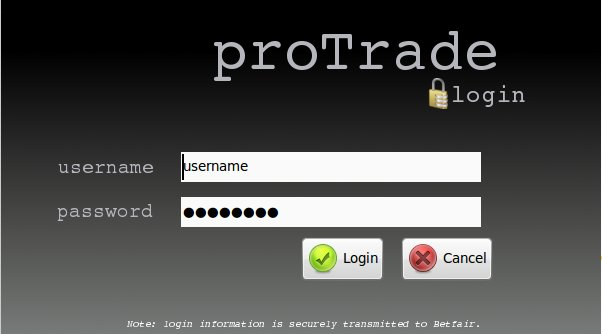
\includegraphics[bb=0 0 650 350, scale = 0.3]{features-screenshots/login.jpg}
\caption{Login screen}
\end{figure}

\subsubsection {Login to proTrade/Betfair}
Implemented at the very beginning of the project, this feature allows for displaying a shell window where the user can input his Betfair account username and password. This sensitive information is then transmitted securely in an encoded format to Betfair using their API authenticator. A neat design based on simplicity and an added progress bar, wrap around this functionality, to enable an easy entry point to both the user's Betfair account and the proTrade application.
\subsubsection {Cash balance and profile preferences}
The Betfair account cash balance can be managed directly from the application, without the need to visit the exchange website. Information retrieved from the betting exchange's API and displayed in the top right corner of proTrade regarding a user's profile includes: current and available balance (currency in AUS or GBP), credit limit, exposure and exposure limit, address info, contact info and timezone. The user can set both a "Display my name" and/or a "Remember me" option for the application to cache his/her personal information.

\subsection {Betfair API information}
\subsubsection {Market access}
A Betfair connection handler maintains a live session with the Betfair servers through the exchange API, using a context wrapper to encapsulate session details (i.e. token). By creating a request object each time information is exchanged, proTrade is able to retrieve information locally for storing or displaying and/or update live account information.
\subsubsection {Market information retrieved}
The market data obtained from Betfair can be broadly categorized into odds market data and set market data. Each market event generated by the API is handled by proTrade to ensure that the user has complete up-to-date knowledge of the match he wants to place trades on. 
\subsubsection {Match Navigator}
\begin{figure}[ht]
\begin{minipage}[b]{5 cm}
\centering
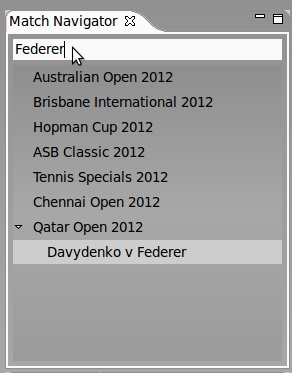
\includegraphics[bb=0 0 650 350, scale = 0.35]{features-screenshots/navigator.jpg}
\caption{Match navigator}
\end{minipage}
\begin{minipage}[b]{7 cm}
Since markets are essentially matches (during their in-play period), a tennis trader needs fast access to the match he wants and is able to enter bets onto. A Navigation Panel allows for search and filtering of matches by player's name and groups them into tournaments. In addition, the match navigator ensures that all matches that it gives the user access to, are current ones, focusing the application only on the live active market.
\end{minipage}
\end{figure}

\subsubsection {Back/Lay spreads}
\begin{figure}[ht]
\centering
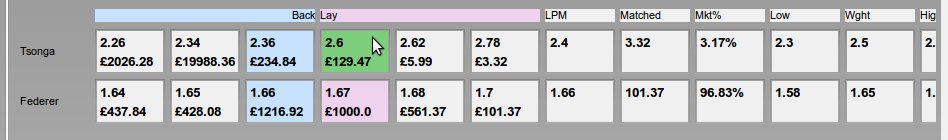
\includegraphics[bb=0 0 950 150, scale = 0.36]{features-screenshots/spread.jpg}
\end{figure}

When receiving market updates related to a specific match, proTrade extracts all information vital to a trader's participation in that market, such as the last matched prices, total amount matched and arrays of back and lay prices and amounts for each player. These are then visualized in a dynamic horizontal array, giving a back/lay spread interface to the market similar to the ones seen in finacial markets, such as the book-keeping tools offered by Fidessa. 

\subsection {Bet placement with history}
From the back/lay spread, the user can open a bet placing window where he/she is able to place a real or virtual bet. After setting the amount and odds to place the bet at, a warning about the potential profit and liability is displayed. Once the bet is placed, it is displayed in an active bets window for easy trading position management.  

\subsection {Live scores}
\subsubsection {Retrieval}
Live scores are essential to both manual tennis trading as much as it is to odds inferring models like the one described below. In the absence of Betfair API or any other free API or feed providing live scores, proTrade fetches scores by web-scraping information from www.livexscores.com. A headless automated browser created through a separate library connects to the relevant page of the website, and fetches strings for further parsing.

The above mentioned website is updated directly via an encrypted incoming connection to the official ATP score feed, that is in turn updated by the umpire chair electronic system present at any match. The score extraction method is indirect and thus poses some delay problems which are difficult to precisely estimate(in the interval 10-30s). Due to encryption, a direct feed from ATP has not been possible, unless advanced image processing techniques are used. However, this is beyond the scope and time frame of our project, but may constitute the subject of further research.

\subsubsection {Constant updates}
As changes in score occur frequently and at undefined intervals of time, a separate thread has been created to poll online for live scores at every 5 seconds, and if a change has occurred, to propagate it throughout the application.


\begin{figure}[ht]
\begin{minipage}[b]{7 cm}
\subsection {Historical statistics}
Historical player statistics are obtained by proTrade for the protagonists of the in-play match the user looks at. Detailed statistics include basics, match and serve statistics (used in odds inferring), and are obtained in a similar manner to live scores, using the website www.tennisinsight.com  as a source to search for relevant information.  
\end{minipage}
\begin{minipage}[b]{5 cm}
\centering
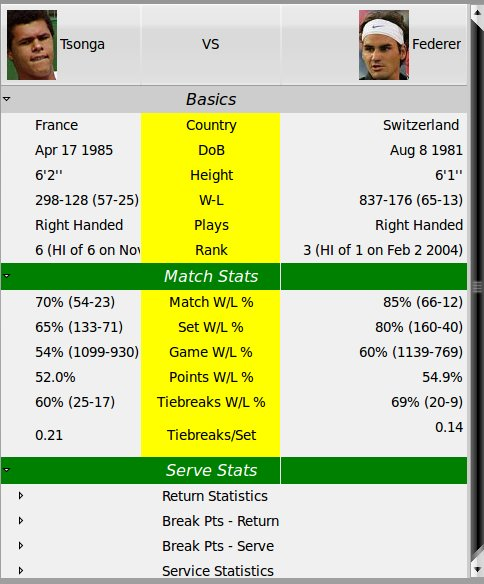
\includegraphics[bb=0 0 650 600, scale = 0.30]{features-screenshots/stats.jpg}
\caption{Statistics panel}
\end{minipage}
\end{figure}


\subsection {Model for odds prediction}
\subsubsection {Markov chains}
Market odds for a specific match are predicted using Markov chain models that use as input the current live score and serve statistical player information. The model used is described in a number of academic papers focusing on tennis modeling, such as Wozniak, Barnett, and Huang. Due to brief descriptions of interest and one-sided formulas, all sample data found in the papers outlined above has been used in extensive testing of the model implementation, in order to validate its correctness. Recursive formulas are derived for describing the probabilities of a player winning a match, in a bottom-up fashion, so that each point registered at a specific score, in a match between certain players, is reflected in a different proportion on the overall probabilities of winning the match (the odds of the match).
\subsubsection {Game}
We model the advantage game as a Markov chain of different point score combinations, and our underlying measure of player performance is the probability of winning a point on serve. The latter is derived from a players' statistics on both his first and second serve, whilst the updated score provides a correct point score to identify the state of the chain at the present time. A tiebreaker game, on the other hand, is modeled following a different recursion, similar to set level, as outlined in Barnett. A major factor contributing to game level probabilities and eventually inferred odds is the static nature of statistics, not entirely reflecting current player shape on the match day. A more dynamic model can be built, inferring statistics from the on-going match, but it would require a long calibration time as a negative trade-off.
\subsubsection {Set}
The set level is modeled via recursive formulas with boundary conditions as explained in the cited papers. However, a distinction must be made between matches with a final set ending in a tiebreaker or simply a continuous advantage set. This input will be set on a tournament-to-tournament basis, as set out in the rules accompanying them. A further current set formula is implemented to reflect any point score change in the current game.
\subsubsection {Match/Odds}
Finally, a win-match formula is implemented recursively based on the current set formula and a match winning probability derived from a Markov chain of advantage/tiebreaker sets.


\subsection {Market Data Plotting}
\begin{figure}[ht]
\centering
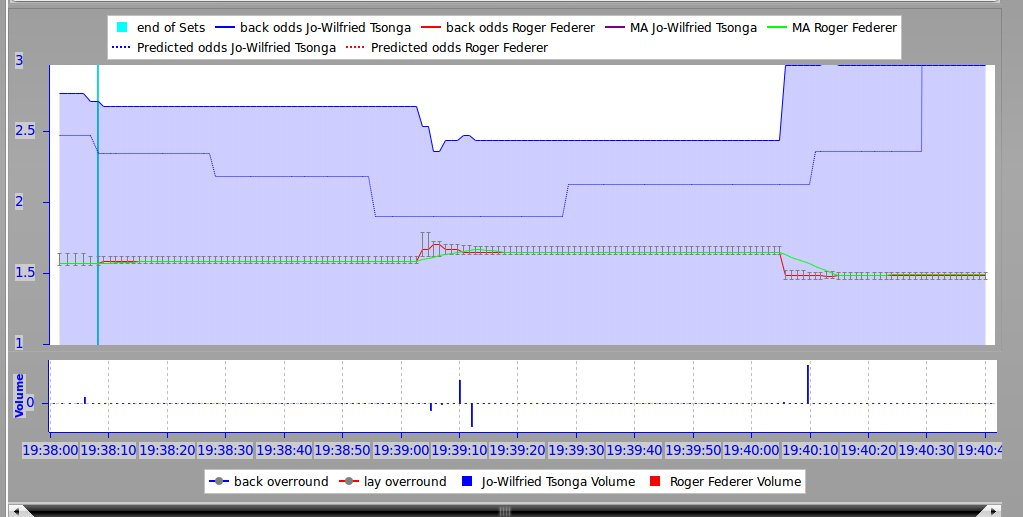
\includegraphics[bb=0 0 1100 350, scale = 0.34]{features-screenshots/chart.jpg}
\caption{Chart with volume traded, back and predicted odds for Tsonga and back odds, MA, and spreads for Federer}
\end{figure}

\subsubsection {Market Odds}
A chart display widget has been built to plot market odds retrieved from Betfair, both back and lay, for both players. In addition, moving averages, back-lay spreads, and the predicted odds for both players can be visualized on the chart as well. The user has also the option to toogle between decimal and percentage plotting of odds. A chart settings window can be opened to choose between an area, anti-alias or step chart drawing schemes for different data. From the same window, default colors can be set to any sequence of values. A legend above the chart will display the current color settings.
\subsubsection {Volume}
Volume is plotted in the same widget, under the market odds chart, and gives the tennis trader a representation of the magnitude of the market reaction to certain events occurring during a match.

\subsection {Match data recording/playback}
\subsubsection {Fracsoft/Variable speed}
Though the importance of running a live match with all its data through proTrade is relevant to real trading, the ability to run recorded matches is vital for further inspection and research of trading patterns, match evolution and virtual bets. Therefore the latter becomes an essential tool in the continuous learning curve of the professional tennis trader. The project identified Fracsoft as a source of recorded tennis match data, which can be visualized in a limited manner on their website. By adapting our own formats and representation of live data to fit with the recorded format under a common interface, proTrade is able to replay a match recorded in a Fracsoft file, fetching missing information(i.e. statistics), to replicate a live match. This can be done at a variable speed, that is synchronized on all information channels.  
\subsubsection {Recording}
After starting with playback, the development of proTrade added recording functionality for in-play matches, which has been successfully tested on the 2011 ATP World Tour Finals final match (Federer-Tsonga).   

\subsection {Configurable dashboard}
A dashboard has been created to support easy creation and display of new widgets. It also provides a more robust and centralized way of managing widget interaction with the user, such as resizing or moving and allows for a standardization of widget behavior.

\subsection {Video Feed}
A live video transmission of the in-play match of interest forms part of the application, as it plays a vital role in recognizing won points earlier on, and is a useful visual tool to be used in conjunction with the scores and market odds of both live and recorded matches. However, the main difficulty encountered is the lack of a source of free tennis match broadcasting, having an easy search and filter functionality.

\subsection {Internal browser}
For more details on player rankings and all other ATP-related extra information, an internal browser can be open as a new widget and will point directly to the official ATP website.

\section{Challenges}
\subsection {Lack of free APIs}
\subsection {Multi-threading issues}
\subsection {Data management}
\subsection {Validating odds prediction}


\chapter{Software Engineering Issues}

This chapter discusses how important aspects of Software Engieering were tackled.

\section{Technical Challenges}

A number of technical problems were generated by the unavailability of free tennis statistics. This has lead to an intricate and computationally intensive solution for obtaining the data, which in turn has lead to a shift towards a multi threaded architecture with all its associated complications.

All these issues have been overcome, as described in detail below, without significantly impacting the ability to deliver core functionality (and extensions) on time - a more detailed estimation is presented in sections \ref{schedule} and  \ref{estimating}.

\subsection{Dependencies on Third parties}
The lack of a central source for all the required data (market data, live scores and tennis statistics) has generated significant dependencies on external service providers. Furthermore, some data sources are very unreliable (e.g. data obtained by parsing web sites - as described in the next section).

The current solution is to design independent and resilient user interface components, such that if one fails or is delayed in fetching data, others remain functional and responsive.

\pagebreak
{\bf This page is intentionally left blank.}
\pagebreak

A long term solution aimed for iteration 8 is to move the logic for fetching live scores and tennis statistics (the major source of unreliability) to a remote server that provides a clean interface exposing all required data. Unfortunately, the Betfair certification program prevents us from additionally providing Betfair market data through this interface.

This architecture could offer an increase in performance and better stability for the desktop clients, but would add the complexity of another transport layer and also complicate the build process (since it would effectively lead to a separation into two projects).

\subsection{Lack of Free Tennis Statistics}
The unavailability of free data for player statistics has proven itself a major issue, forcing us to resort to data obtained from www.tennisinsight.com, by paying a small fee to get access to this comprehensive tennis statistics website. 

Though the method to fetch data is similar to the one employed in fetching live scores (detailed in Report One), additionally, we need to automatically execute some functionality of the website, like logging into our test account and navigating to the relevant player head-to-head comparison (for the currently selected match). This is achieved using the Rhino Engine included in HtmlUnit, which is able to natively execute Javascript and intercept its execution to collect data, allowing us to scrape the page we are interested in. Though the original intent of the HtmlUnit Java library is to unit test website builds, it can effectively be used to scrape information from live websites, mimicking the functionality of an automated headless browser. However, as detailed above, extensive data fetching poses more challenges to having a reliable and responsive application.

Obtaining this data is particularly important to the project because, aside from constituting a good source of information for the user, both live score and player statistics are to be used as inputs to a Markov chain model capable of accurately predicting live odds for the next point, set or entire match. This model will be integrated with our application and have all its outputs visible, as well as the predicted match odds displayed along the real ones on the graph. The user will thus be able to compare the prediction with the actual odds evolution and form opinions on possible trading arbitrage situations that may occur at any in-play time.

\subsection{The Switch to a Multi Threaded Architecture}
Because the task of fetching and parsing data is computationally intensive, as described above, we have decided to shift to a multi threaded architecture, splitting existing functionality into a user interface thread and a number of processing threads (responsible for fetching and processing data).

This architecture allows for a responsive user interface even in the (very likely) situation in which data is not available (e.g. if the network connection goes down) and is the foundation for the resilient and independent component model mentioned previously.

The separation achieved between user interface and logic should prove very  useful in iteration 8, facilitating the shift to the client server architecture.

\subsection{Threading Issues}

The shift to a multi threaded architecture has generated a few issues by itself.

The most significant one was related to the SWT threading model (apartment model), which does not allow updates of user interface components to be carried out from other threads than the user interface thread. This problem has been overcome through careful design, but required a more in depth understanding of the framework than we had initially anticipated.

Furthermore, it has become increasingly more difficult to reason about the correctness of the application (as in any multi threaded programs), which has led to an increased number of bugs. Although, so far, most have been rather obvious (e.g. hanging the user interface indefinitely), the team has decided to adopt more rigorous methods for spotting errors in order to prevent them from propagating to production code.
Namely, we intend to make even more use of pair programming, functional and unit testing in upcoming iterations.

Performance might also constitute an issue, particularly on single core, old generation CPUs. This concern has lead to the need for a more rigorous benchmarking approach, which should (at a minimum) provide some rough indicators of the performance of the application (number of threads, CPU utilisation, memory consumption, object instances etc). This is discussed in more detail in section \ref{perf}.

\subsection{Build Issues}

Currently the project uses a number of classes automatically generated from large WSDL specifications which are approximately 400 thousand lines long (just for the Betfair API).
This has generated a serious increase in compilation time due to some inefficiencies in the build script (e.g. a "run" performed a "clean" before recompilation).

Since the specifications are not expected to change often, the compiled classes have been packaged into a library, effectively removing the need for recompilation.
A task which automatically generates the classes, compiles, packages them and updates the library has benn added, should this be required in the future.

\pagebreak
{\bf This page is intentionally left blank.}
\pagebreak

\section{Risks}

We have classified potential risks into three main categories:
\begin{itemize}
\item Technology risks
	\begin{itemize}
		\item initially selected APIs do not provide adequate functionality
		\item critical APIs (e.g. Betfair) are hard to use
		\item other selected APIs (e.g. SWTChart) are hard to integrate
	\end{itemize}

	\item Team risks
		\begin{itemize}
		\item different work ethics among team members
		\item different coding practices among team members
	\end{itemize}

	\item Other risks
		\begin{itemize}
		\item hard to predict team member's availability - (e.g possible interviews for Industrial Placement, coursework deadlines)
	\end{itemize}

\end{itemize}

\section{Collaboration}
Any collaboration/coordination difficulties encountered and how addressed 

\section{Development Methodology}

The team has decided to adopt a more rigorous development methodology, more aligned with Extreme Programming, as described in \cite{extremep}.
For this reason, a more specific set of practices will be adopted, which is expected to further improve productivity and communication between team members.

More rigorous estimation and performance measuring methods are also discussed.

\subsection{Practices}

A table summarizing the practices (as found in \cite{extremep}), whether they have been adopted or on course to be and the expected benefit or other observations is presented below. A number of practices are included in section \ref{manag}, so they are not covered here.

All practices should result in better cooperation and increased productivity so this is not included in the table.

{\bf Legend:}
\begin{description}
\item [Yes(n)] - applied beginning with iteration n 
\item [No(n)] - not yet applied, but should be applied no later than iteration n 
\end{description}

\begin{center}

\begin{tabular} {p{2.25cm}|p{4.5cm}|p{1.5cm}|p{5cm}}
{\bf Practice} & {\bf Short Description} & {\bf Applied} & {\bf Outcome / Observations}\\
\hline

Stories & "Plan using units of customer visible functionality" \cite{extremep} & Yes(0) & Providing earlier estimates would be beneficial. \\
\hline

Ten-Minute Build & Build the whole system and tests under 10 minutes. & Yes(0) \\
\hline

Continuous Integration & "Integrate and test changes after no more than a couple of hours." \cite{extremep} & No(5) & Helps identify errors or bugs  as soon as they are introduced.  \\
\hline

Test-First Programming & Write a failing automated test before changing any code. & No(4) & Helps avoid "scope creep"; improves coupling and cohesion;
improves trust and rhythm \\
\hline

Shared code & Any member can improve any part of the system at any time. &
Yes(2) & Risks include people acting irresponsibly (if they are not responsible for the particular piece of code) \\
\hline

Code and tests & Maintain only code and tests as permanent artifacts. & Yes(1) & Generate all documentation from code. \\
\hline

Single code base & There should be only one code stream and single branches shouldn't live for more than a few hours. & Yes(0) & A single master branch.
Only keep code for current release. \\
\hline

Daily Deployment & "Twelve releases sounds a lot better than twelve patches." (\cite{extremep}) & No(6) & Lack of continuous integration represents a technical barrier \\
\hline

Pay-per-Use & Charge every time the system is used & No(8) & Charge a base price for the application and then charge a small amount for individual widgets.

This provides good feedback on which widgets are actually useful/desired.

\end{tabular}

\end{center}

\subsection{Testing}

In terms of testing, particularly important are the "Test-First Programming" and "Continuous Integration" practices. These have not been applied so far due to lack of familiarity with testing APIs but also with other libraries. However, we have developed tests for the main classes, containing most of the business logic of our application.

After researching \cite{testing} and gaining a better understanding of the test-driven approach, we believe we have gained enough confidence to start  gradually applying the "Test-First Programming" practice, beginning with the next iteration.

Also, a continuous integration server will be deployed in the following iteration, since the application has reached a state in which errors can be easily introduced. This practice ensures any new bug can be quickly identified, at which point solving it becomes the priority - temporarily suspending other commits form taking place.

\subsection{Refactoring}

Refactoring has been applied frequently in order to improve code quality, which has lead to increased productivity. Most common applications such as method extraction have been at the heart of a continuous process which aimed to maintain code readability. Furthermore, large classes have been refactored to achieve decoupling between application logic and application UI.

A major redesigning of the code is intended to take place in iteration 4 in order to facilitate the introduction of the story "Record odds and data into .csv file" (Fracsoft format).

To ensure this progresses without breaking existing functionality, refactoring will be applied extensively.

\subsection{Planning and Estimating}
\label{estimating}
We are only using the primary indicators (described in Report One) as a reliable project measure - secondary indicators are just to give an overview of some important aspects of the project.
User satisfaction is high.
For measuring team velocity we take a moving averege of the last three iterations (as suggested in \cite{estim}), which leads to a velocity of 30. Further, we allow a margin for error, taking an interval around this average velocity which leads to the range 26-34 (\cite{estim}).

A burndown chart is used to rapidly indicate whether at the current velocity, the team is on schedule.

\begin{figure}[ht]
	\centering
	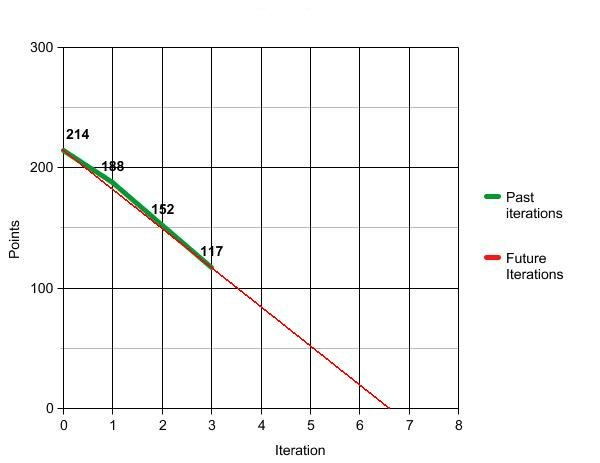
\includegraphics[bb= 0 0 400 400, scale=0.65]{graph.jpg}
	\caption{Burndown chart}
\end{figure}

Currently, we are expecting to finish before the begining of the 8th iteration, which allows additional time for unexpected issues, polishing or even addition of extra features.

\subsection{Benchmarking and Performance Measuring}
\label{perf}

As described above, because of the number of threads created by the application, it is important to test it on older generation, single core CPUs, which might experience a significant decrease in performance.

Currently we are researching into profiling tools such as the Eclipse Profiler, Netbeans Profiler, MemCheck, Cachegrind and the JVM Profiler Interface. These are aimed to help identify memory leaks and a number of runtime statistics (memory and cpu consumption, number of threads and object instances created, number of native objects created etc.). This is especially important due to the architecture of SWT, which, via native calls, creates instances which might not be garbage collected even at application shutdown.

It is hoped that profiling can be integrated with unit and functional testing by the end of iteration 5, creating the possiblity of running automated performance tests, which could, for example, start and close the application a large number of times asserting that memory consumption has not increased significantly.

\section{Testing}
\label{sec-testing}

We started to use testing as soon as the first cohesive draft of the Match API, containing all core features, was created (iteration 3). This allowed us to validate our design and do any major refactoring work around that stage. From the beginning of iteration 5, testing has been supplemented with continuous integration and measuring code coverage to ensure a continuous monitoring of the state of the project. After obtaining all necessary data for building the Prediction API, further tests were developed along the way, leading to a TDD approach for the latter part of the project.

As suggested in \cite{bk-testing} we have used the tests to guide our design, based on the principle that if a project is well designed it should be easy to write meaningful tests for it.

\textbf{Unit testing} has been used to rapidly test small portions of code while \textbf{acceptance tests} have been used to test a system feature from front-end to back-end. \textbf {TDD tests} (tests written before features) are expected to fail when they are written and should pass once the feature has been completely implemented. Once it passes, a test is transferred to the regression suite. Naturally, a failing \textbf{regression test} indicates a break in previous functionality (regression).

The general approach was to use TDD for the model packages, based on the fact that these should be easier to test, are crucial for the application and less likely to change.

Because of the lack of familiarity with the UI libraries and the limitations and lack of documentation of the UI testing framework - which could have threatened the ability to deliver the project on time - we avoided a TDD approach for the UI classes, but resorted to writing post implementation acceptance tests to cover a decent proportion (generally over 60-70\%) of the user interface functionality.

\subsection{Unit Testing}
Unit testing was adopted early on in the development process and it has been of great use in identifying bugs and ensuring correctness of the Match API (an important set of classes which manages data such as match score and statistics). 

One specific use case was to test the implementation of the scoring rules. Since, in tennis, these can be quite peculiar (for example points are counted 15, 30, 40, AD instead of just 1, 2, 3, 4) and tests are particularly easy to write, we adopted a TDD approach in this instance. A simple initial test was written to state the expected outcome of adding four consecutive points to one of the players: the player in cause should win the game, increasing his game score, and resetting the points score. Furthermore the opponent's score should always be zero. The code for this is presented in Listing \ref{list1}.

\javalst{Initial failing test for score. The initialisation of the score object is handled in an abstract super class which also provides assertSetScoreIs() and assertGamesScoreIs().}{list1}
\begin{lstlisting}
  @Test
  public void fortyZeroWin(){
    int expectedPoints[] = {15,30,40};
    for (int i=0;i<3;i++){
      score.addPlayerTwoPoint();
      assertGameScoreIs(0,0);
      assertPointsScoreIs(0, expectedPoints[i]);
    }
    score.addPlayerTwoPoint();
    assertGameScoreIs(0,1);
    assertPointsScoreIs(0,0);
  }
\end{lstlisting}

Having first written the test and ensured it failed, we then proceeded to designing and implementing a solution that would make it pass. We adopted this approach for the whole Match API and for the Prediction API (used to predict the evolution of a match based on current score and player statistics).

This approach helped us identify numerous bugs early on and guided us towards a better overall design of the APIs. For example, a function for correctly setting a set score to a certain value was not initially provided, but since while writing the tests the need for such a function became obvious, it was included and tested.

\subsection{Acceptance Testing}

We used acceptance tests to test a particular function of the system, starting
from the front-end (e.g. finding and pushing a button on the UI) to the back-end
(e.g. connecting to the Betfair API to authorize a login request).

For performance reasons these were ran separately from unit tests since the UI
operations tend to be slow.

A simple example is the test in Listing \ref{list2} which checks the login functionality:
the user should fill in their Betfair account and password and click on the login
button. The login attempt is checked against the Betfair API and a label is
updated to indicate success or failure. Obviously, an attempt to login with the
specially created test account should result in a success message being displayed.

We have adopted a similar approach in testing most of the classes connected to
the user interface.

\javalst{Initial failing test for the login window. The username and password for the test account are read and decrypted from a local config file by the Main class. Using the UI bot we then fill the data in on the login window and click the login button. Similar tests have been written to verify other scenarios.}{list2}
\begin{lstlisting}
    @Test
    public void correctLoginSuccess() throws Exception {
        SWTBotText username = bot.text("username");
        username.setText(Main.getTestUsername());
        SWTBotText password = bot.text("password");
        password.setText(Main.getTestPassword());
        loginButton.click();
        SWTBotLabel success = bot.label(LoginShell.SUCCESS);
        assertNotNull(success);
    }
\end{lstlisting}

However, due to limitations in the SWTBot API some features have proven impossible to test. For example we have not found a way to test the functions of a context menu (pop up) or a progress bar.
Nevertheless these are important aspects which must be tested to ensure correct behaviour. For example, one of the most important tools for traders is the chart on which they can view the market's evolution. Since a context menu on the chart allows the user to choose between different types of analysis, it is currently impossible to completely test the correctness of this function.

In such situations we have resorted to testing the actions executed by the specific listener associated with the context menu item, which at the very least ensures that if the event fires correctly, the display is updated as expected.

\subsection{Regression Testing}
We have used regression testing to ensure that no break in previous functionality occurs when introducing new code.

Keeping tests that measure progress separate from regression tests is key in quickly identifying when a regression has occured. Simply put, all tests appart from those in the progress suite should pass at all times. If this is not the case, a regression has occurred.

Consequently the normal development flow is: 
\begin{enumerate}
\item write a failing test (and ensure it fails)
\item make the test pass
\item check for regressions
\item fix any regression
\item move test from progress suite to regression suite
\item commit changes
\item repeat
\end{enumerate}

\subsection{Integration Testing}

Given the dependency on a large number of external APIs, we have used integration testing to ensure that these behave as expected and quickly identify potential configuration issues. 

This has been done by writing tests that ensure the abstractions built on top of the libraries work as expected. To reduce coupling (and simplify the testing process), normally one interface and an implementation class expose the required functionality, encapsulating all other logic required for manipulating the library. As examples we discuss the testing approach for three of the most heavily used libraries: the Betfair API, SWT and SWTChart.

\subsubsection{Betfair API}

The Betfair API is organised in three services: global, UK Exchange and AUS Exchange, each defined through a WSDL specification. The application only uses the first two services, accessing them through Java classes automatically generated with Apache Axis.

Any connection to Betfair and use of the API is handled by classes in the src.model.connection package. Moreover, to ensure both services (Global and UK Exchange) only have one point of access, all the functionality required by the application has been encapsulated in two classes - BetfairExchangeHandler and BetfairConnectionHandler. Hence, tests written for these classes ensure the connection to the Betfair API works as expected and constitute integration tests.

\subsubsection{SWT}

SWT is a graphical widget toolkit with a platform dependent implementation. At the heart of its architecure is the ability to create native widgets. However this raises the issue of freeing allocated memory (which cannot be garbage collected by the JVM).
Hence, it is important to test classes using this library(most of our UI classes) to ensure that the UI behaves similarly on different platforms and that there are no memory leaks.

However, precisely matching UIs for different platforms and reliably identifying memory leaks have proven to be very difficult tasks, so we have postponed handling of these aspects to later stages.

In all other respects, we have considered the acceptance tests as good enough to test integration with the SWT library.

\subsubsection{SWTChart}

The SWTChart API provides a chart component with several basic functionalities (such as drawing line functions, bar charts etc). The chart can handle real-time updates (even for large data series), which is crucial to the purpose of our project and, since it is based on SWT, it integrates smoothly with the application's UI design and implementation. 

The addition of new functionalities requires extending the Chart class. This design encapsulates the use of the SWTChart API, so integration tests for this class ensure the library integrates well with the rest of the application. 

\subsection{Continuous Integration}

Starting with iteration five, the continuous integration server became a key element in monitoring project evolution with a view towards understanding and adapting to development trends.

\subsubsection{Configuration}
A continuous integration server has been installed on a virtual machine provided by the Computing Support Group, which emulates a dual core, 1GB memory, 64bit machine, running Ubuntu 11 (these details are important due to the platform dependent nature of the SWT library).

We have used Hudson since - unlike other CI solutions - it comes with a plugin for running UI tests on a headless server. This was an important requirement since, in order to run correctly, all acceptance tests must connect to a display instance. (Another alternative would have been to use xvfb -X virtual frame buffer - which buffers display data in memory and works for any application).

Additionally, Hudson presented a few other advantages such as smaller installation size, good out-of-the-box support for git repositories and an easily configurable build management process.

The CI server is set to poll the repository and, when changes are detected, checks out a fresh copy and runs the normal build script. As an extension, since the VM is not accessible from outside the local site, a step to move reports and artefacts to a publicly accessible location (group directory / home directory) has been added in order to simplify the process of checking the build status.

The build process generates reports for unit tests, system tests, code quality (discussed in section \ref{sec-quality}) and test coverage as well as historical build trends (e.g. duration).

\subsubsection{Reporting}
\label{sec-reporting}
The reports generated by the CI server were important in understanding the historical evolution of the project. For example, the build duration statistics allowed members to easily understand if the ``ten minute build'' rule is enforced.

Monitoring build ``colour'' revealed the need for a more established code review system. For example, the points where the build is red (45 - 49, 53 - 55, 63 - 66) coincide with periods slightly before supervisor meetings or other presentations and reveal that developers tend to break the build in such crucial moments, most likely, as a result of their desire to contribute last minute additions. Fortunately, the team was able to fix these issues in time but decided nevertheless that such situations must be avoided. As a result, a more rigorous code review mechanism was adopted (presented in Section \ref{sec-codechange}).

\begin{figure}[ht]
\centering
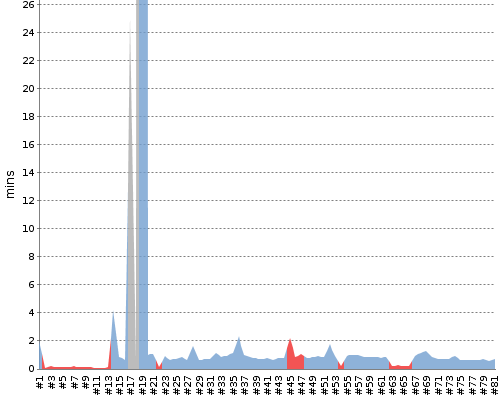
\includegraphics[bb=0 0 500 400, scale = 0.5]{build-trend.png}
\caption{Build trend summary. Vast majority of builds are well under 10 minutes. Outlying values were caused by a network outage.}
\end{figure}

\subsection{Measuring Test Coverage}

Since we did not adopt a TDD approach from the very beginning, it was important to obtain an overview of the parts of the code that required testing. Starting with iteration 5 we have used Cobertura,  an open source tool which provides neat test coverage reports for Java programs.

To facilitate report generation, a single ant task has been set up to compile the code with the debug info (vital for Cobertura to indicate line numbers and measure coverage), run all the tests (unit, acceptance, integration) and generate human readable reports which provide an indication of the current test coverage as well as branch coverage and complexity measures.

The coverage reports enabled us to identify lines which were not touched by tests. This was usually fixed by writting another test to cover the specific path, but it could also have been the case that the functionality was actually never required, in which case it was completely removed. Again this illustrates how tests have been used to ensure we are running a healthy codebase.

\begin{figure}[ht]
\centering
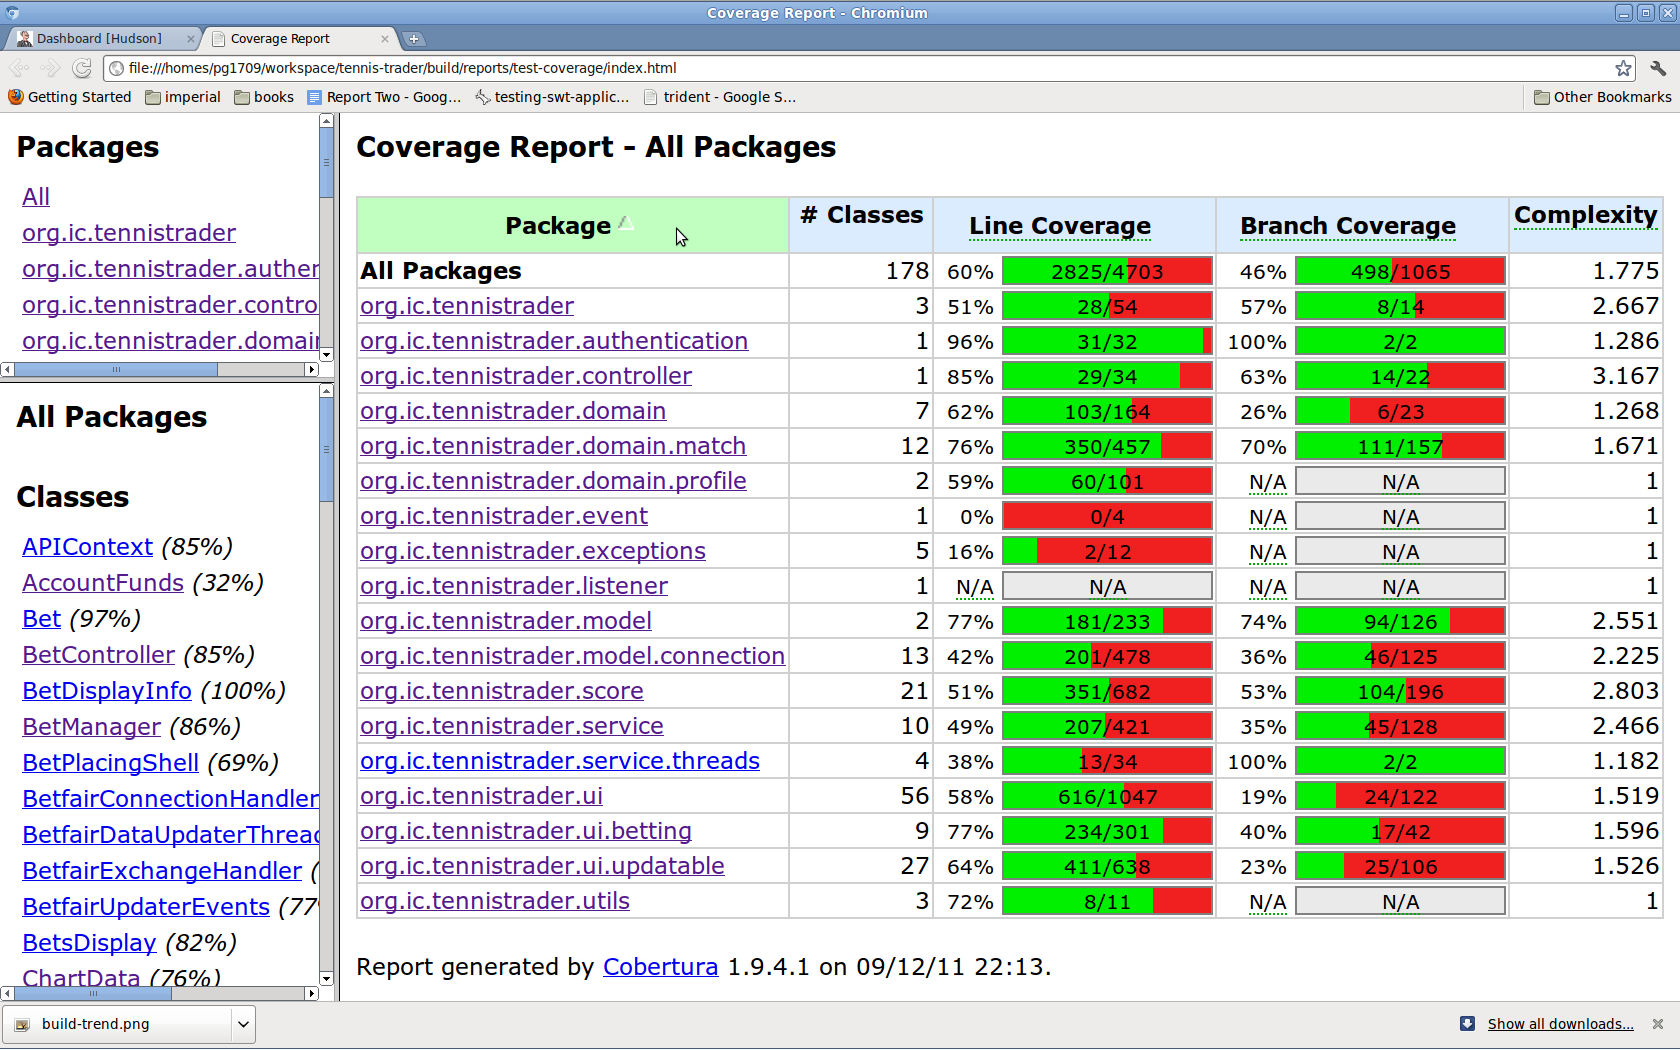
\includegraphics[bb=0 0 1680 1050, scale = 0.2]{coverage.png}
\caption{Coverage report generated by Cobertura indicates test coverage at package level, branch coverage an cyclomtic complexity.}
\end{figure}

Branch coverage indicates when tests do not cover particular cases and has proven useful with regards to particularly tricky conditionals.

Cobertura also generates cyclomatic complexity values for each class/package, measuring the number of independent paths through the control flow graph of the code. Since it has been shown that high values are usually an indication of error prone code ([2]) this measurement is used to check code sanity.

\begin{figure}[ht]
\centering
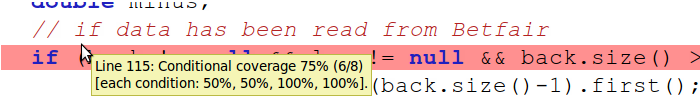
\includegraphics[bb=0 0 700 100, scale = 0.49]{branch.png}
\caption{Branch coverage indicates specific condition coverage.}
\end{figure}

\subsection{Code Quality Measures}
\label{sec-quality}
We have used PMD to generate code quality reports. Additionally we have researched and are looking forward to using FindBugs - a tool which identifies bugs in Java code (such as NPEs and potential out of bounds accesses).

\begin{figure}[ht]
\centering
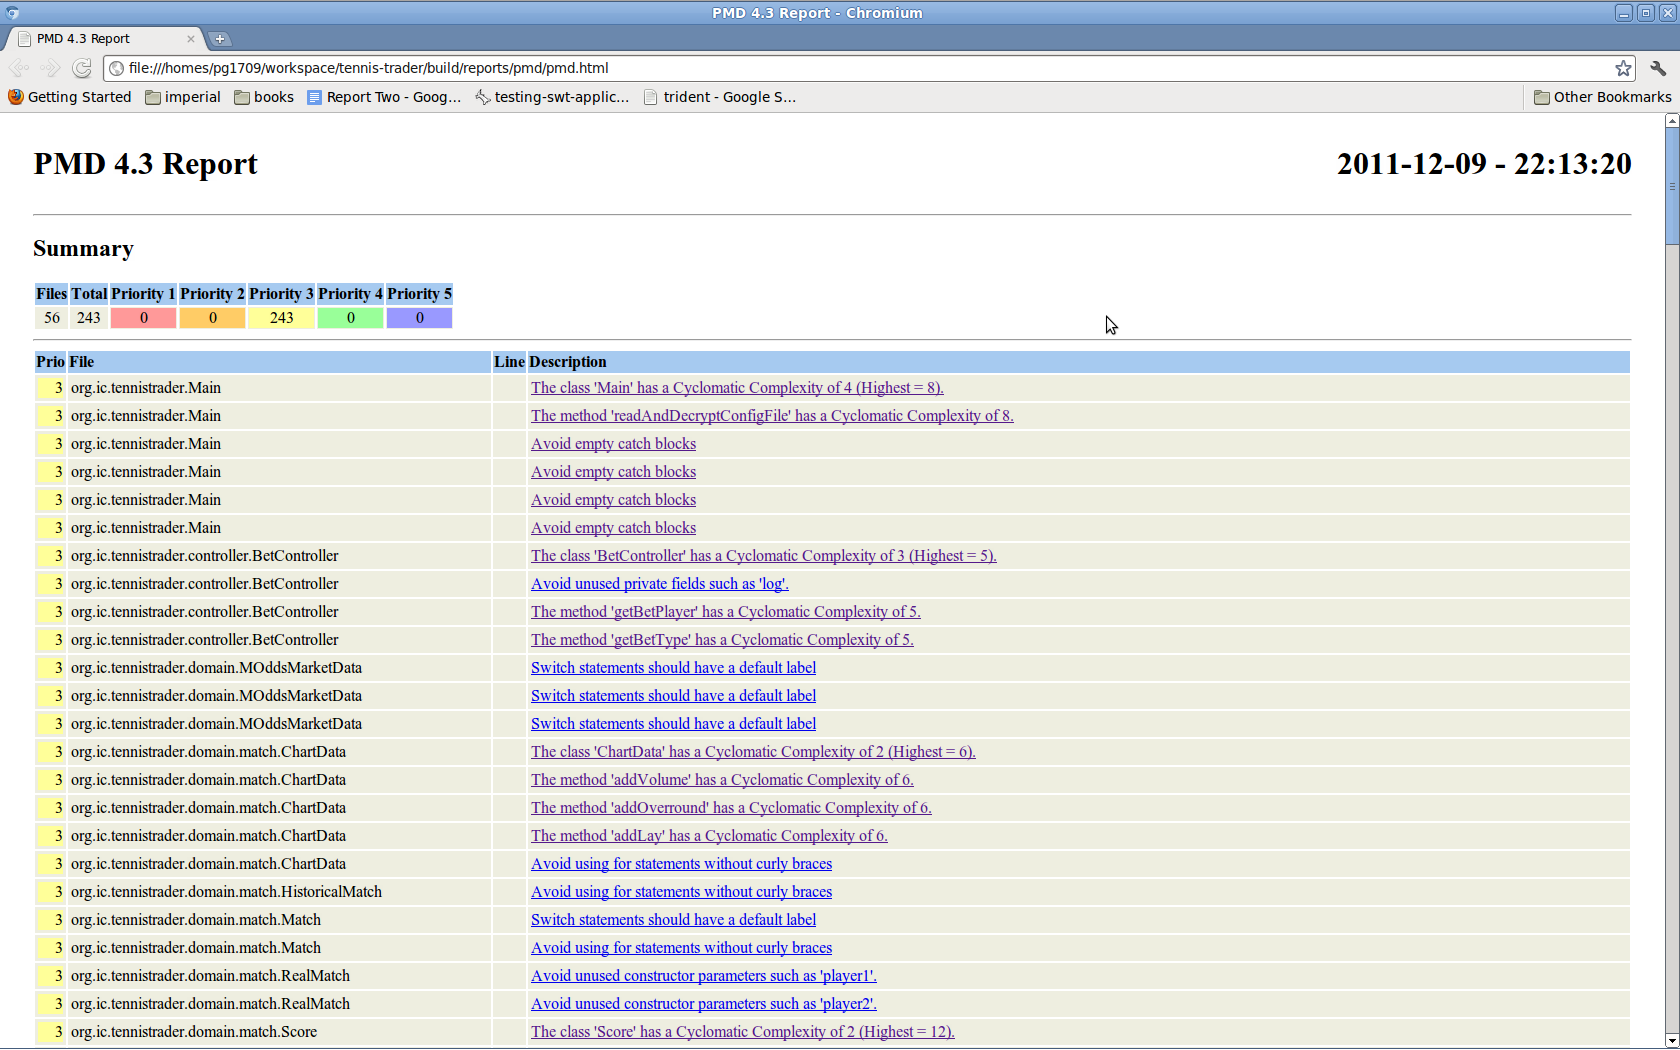
\includegraphics[bb=0 0 1680 1050, scale = 0.2]{pmd.png}
\caption{PMD reports indicate potential quality issues. The tool can be configured to signal a large number of potential issues and comes with predefined rules for optimizations, unit tests, unused code etc.}
\end{figure}

\subsection{Testing Overview}

All core components of the application follow the MVC pattern and this is reflected in the structure of the tests, with unit tests validating the back-end (Model) and functional/acceptance tests verifying the view and controller layers (incidentally acceptance tests also touch model functionality, but their overal scope is broader). Additionally, integration tests are used to reproduce and analyse behaviour of specific libraries. A functional overview of the application’s code base and features together with their tests is given below for subpackages of org.ic.tennistrader.

\begin{figure}[ht]
\begin{center}$
\begin{array}{ccc}
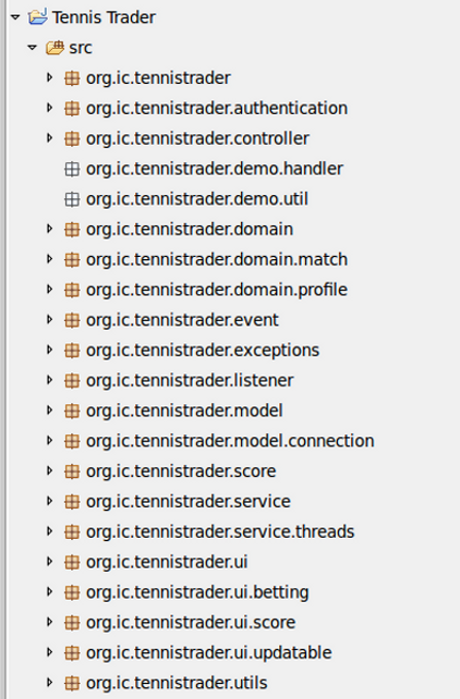
\includegraphics[bb=0 0 499 700, scale = 0.25]{project.png} &
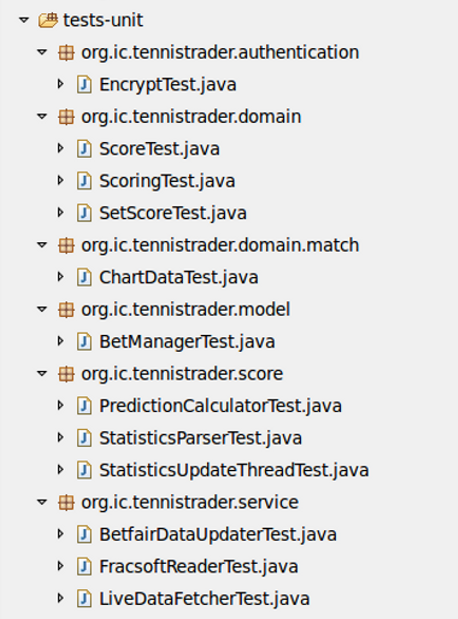
\includegraphics[bb=0 0 499 700, scale = 0.25]{tests-unit.png} &
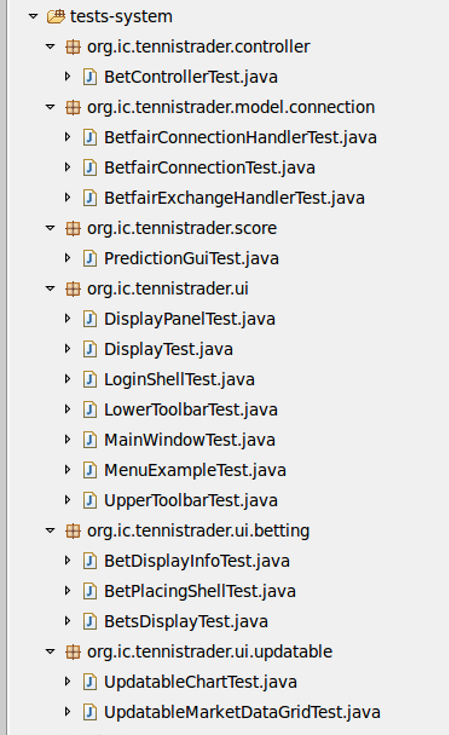
\includegraphics[bb=0 0 499 700, scale = 0.25]{tests-system.png} 
\end{array}$
\end{center}
\caption{Left - Project hierarchy with included packages. Center - Unit tests for local functionality/model based classes/packages. Right - System tests for controller/UI oriented classes/packages}
\end{figure}

\begin{itemize}
\renewcommand{\labelitemi}{$\bullet$}
\item .authentication: Encrypt/decrypt functions for storing and accessing the login credentials are unit tested, while the interface (LoginShell) is acceptance tested (as detailed in section 2.2).
\item .controller: The bet controller, built upon relevant back/lay buttons and their associated bet placing functionality, is tested for correct bet types and player recognition.
\item .domain: Local functionality of populating/retrieving the chart widget with market data is unit tested in 'ChartDataTest'. Specific tests for other domain classes have not been designed, since these are plain java objects, with no logic implementation. However, their functions are tested when these objects are used in other unit-tests.
\item .domain.match: Special unit-tests have been designed to check how the score of a match is updated and handled.
\item .model and .model.connection: The implementation and logic of virtual betting (including the internal state representation of the market and matched/unmatched bets) are unit tested, while the global and exchange connections to Betfair API (that normally update the internal state) are validated via integration tests.     
\item .score: Front end 'PredictionGui' controller is functionally tested, whereas specific unit tests are written for back-end components such as statistics fetching and parsing or the 'PredictionCalculator' model. 
\item .service: Since this package models the back end receiver for various incoming data, state updating is unit tested.
\item .ui and .ui.betting: Acceptance and testing of all front-end GUI interfaces.
\item .ui.updatable: Acceptance and integration testing on dynamical GUI elements driven by user input or data updates.
\end{itemize}

\subsection{Bugs Revealed by Testing}

Apart from validating design, testing has revealed hidden bugs in various components of the system at all tiers of the application. Below we summarise a few examples.

Unit tests have invalidated a first encoding of the scoring system for the prediction calculator, when translating between traditional tennis point scores and an incremental representation.

Also, they have identified a missing condition when registering events whose market data should constantly updated by connecting to the Betfair API, which resulted in some events being introduced twice.

Furthermore, they have revealed some overlooked considerations in recursive state passing when computing a set prediction based on a Markov chain model, which led to wrong set winning probability estimates. 

\clearpage

\section{Comparison of Plans with Actual Achievements }

\section{Effort}
Present estimates of length of code in each of the components, or any other comparable measure of the effort required.

\section{Contributions}
Summary of each team member's contributions 


\chapter{Validation}

We have used validation methods to ensure that the product accomplishes its intended requirements.

\section{User interface design validation}
The user interface of our application has been designed with a view towards
obtaining a final product which achieves the following goals: being visually
eye-pleasing and simple to use, and at the same time minimizing the effort it
takes for users to accomplish their goals. To the purpose of validating our user
interface design, feedback has been collected from a number of different persons
with or without experience in using trading applications.

\subsection{Feedback from Experienced Users}

Firstly, we have had constant feedback from our supervisor, who is familiar with the game of tennis and the world of tennis betting and who understands the needs of a professional trader. He has guided us through the process and has pointed out a number of possible UI improvements along the way (such as positioning different components, displaying different data on the graph), which we have accomplished.
 
Secondly, we have had meetings with PhD students, who are themselves developing trading applications. They provided valuable feedback regarding market information display and the best way to present it to a specialized user. We have collected a number of user satisfaction questionnaires to guide our understanding of the relative importance of such features (see next page for an example). Hence, our initial interface has been adapted to accommodate their suggestions.

Finally, to collect feedback from people in the industry, our supervisor arranged a meeting the Head of Research at Betfair. He has approved of our application’s general interface and pointed out a few possible issues (such as synchronizing all the playback data), which are now fixed.

\subsection{Feedback from Inexperienced users}

To test how easy it is for users to understand the information presented by the application and how ``natural'' it is to find the required functionalities, we have collected feedback from a few colleagues, without previous experience with tennis trading applications and the feedback received was generally positive.

\clearpage
(Left blank for sample user questionnaire)
\clearpage


\section{Code Review}

We also used a review mechanism in which, generally, code has been inspected by at least two team members.

During the implementation process we often employed pair programming but also other lightweight code review mechanisms, particularly over-the-shoulder and tool-assisted code review (e.g. based on PMD suggestions). The decision to adopt lightweight code review mechanisms was based on evidence which suggests that this type of review can be as effective as a more formal one, but easier to implement.

This helped improve the overall quality of the software and minimize the number of bugs early on in the development process. The whole source code is accessible to every member of the group and where appropriate and necessary, the code is reviewed by other members who don’t work on that specific widget or feature. 

Wherever a bug is found or refactoring is needed, an issue is raised on GitHub with the suggestion to solve that specific problem.

\section{Stress testing}

At the moment, no stress testing tools are used. This has been left as the last stage of our development process, as it may be more beneficial once we have all the features implemented. However we have conducted a ``manual'' stress  testing.

An abnormal condition or a stressing condition for our application is when a user tries to view and trade several matches/markets at the same time. This can be done by opening more than one tab, since each tab displays one match and its associated market information.

We have observed that when viewing data for only one match the application’s physical memory consumption is around 1.5 GB, and this can increase up to 2GB (with 3 open tabs). We understand such behaviour is a major problem, as an average computer has 3-4 GB of physical memory, and we aim to solve the problem by the end of the project. Hence, this has become an important issue, starting an on-going process to identify and eliminate memory leaks.

Using the Standard Widget Toolkit (SWT) to develop the graphical user interface can be a source of memory leaks, since the native OS widgets created by it cannot be garbage collected. Therefore, special attention is paid to disposing any created components.

Also, the application requires a lot of data to be stored and presented to the user in different ways. Hence, one of the aims is to have an efficient memory management, as this will avoid having duplicate data in memory.

The application does not require a lot of CPU power as most computations are negligible. The most computationally intensive tasks are the statistical data inference algorithms, but we havent observed a heavy CPU usage even with more match views open at the same time.

\clearpage

\chapter{Conclusions}
  \begin{itemize} 
  \item Was the project successful?
  \item What did you learn?
  \item What might you have done differently?
  \end{itemize}  

\begin{thebibliography}{9}
\bibitem{bk-testing}
  Steeve Freeman, Nat Pryce,
  \emph{Growing Object-Oriented Software, Guided by Tests}, Addison-Wesley 2010

\bibitem{web-cyccom}
  Robert Chatley's course on Software Engineering Methods
  \url{http://en.wikipedia.org/wiki/Cyclomatic_complexity},
  Imperial College London

\bibitem{bk-aglsam}
  Jonathan Rasmusson,
  \emph{The Agile Samurai},
  Pragmatic Bookshelf,
  October 2010.

\bibitem{bk-aglflh}
  Jeff Langr and Tim Ottinger,
  \emph{Agile in a Flash},
  Pragmatic Bookshelf, 
  January 2011.

\bibitem{web-rbc}
  Robert Chatley's course on Software Engineering Methods
  \url{http://www.doc.ic.ac.uk/~rbc/302/},
  Imperial College London

\bibitem{site-fracsoft}
  Site of Fracsoft, authors of Fracsoft Data Viewer
  \url{http://www.fracsoft.com}

\bibitem{site-betangel}
  Site of BetAngel
  \url{http://www.betangel.com}
  
\bibitem{wiki-swt}
  SWT - Wikipedia
  \url{http://en.wikipedia.org/wiki/Standard_Widget_Toolkit}

\end{thebibliography}

\clearpage
\appendix

\chapter{Tennis Rules}

{\bf General}\\
Tennis is played between two players(singles) or between pairs(doubles).
The aim is to win enough points to win a game, enough games to win
a set and enough sets to win a match. Matches are usually played as best of three
sets, but best of five sets are also played in high profile mens tournaments (Grand
Slams). 
The game is played on a court with specific dimensions divided by a net of a specific height.\\
\\
{\bf Service} \\
Opponents stand on opposite sides of the court and players deliver the ball in turn.
The player who delivers the ball is called the server and the player who stands opposite and cross-court from the server
is called the receiver. 
The right to serve or choose the side is decided by a toss of a coin or a racquet.
The half of the court on the player's right side is called the deuce court and the left half is called the advantage court. 
The server shall not serve until the opponent is ready. All even points are played from the deuce court and 
all odd number of points played from the advantage court. The servers are made from the deuce court to the opponent service box
on the deuce court or from advantage court to advantage service box. If the server misses his target twice, he loses the point. 
If the ball hits the net and goes in the correct service box, another serve is granted. If the server steps on the baseline before contact is made, 
the serve is deemed a fault. \\
\\
{\bf The Game} \\
If the ball goes into the net, or outside the boundaries of the court, the player who hit that ball loses the point. If the ball hits the net during the point and goes into the opponents court, the ball is in play. A player loses the point if he touches the net, drops his racquet while hitting the ball, bounces the ball over the net, hits a part of the surroundings such as the roof, or a tree, the ball touches him or his partner, he deliberately tries to distract the opponent.
A ball that lands on the line is good.\\
\\
{\bf Scoring} \\
The server always calls his score first. If server wins the first point, he/she gets a score of 15. The score is done like a clock. Love means zero in tennis.
The second point is called 30. The third point is called 45(now-a-days known as 40) and the game is won when the score goes back to love. If the score is 40-40, 
also known as deuce, one side must win by two points. ( Love-15-30-40). \\ 

The first player to win 6 games by 2, wins the set. If the score is 5-5, the set is played until someone wins 7 games. If the score is 6-6, a tie-breaker is played.
The tie-breaker is scores by one's rather than (Love-15-30-40). The first one to score 7 points by 2 in the tie-breaker wins the set. If the score is 6-6, one side must win
by two points.  \\
Usually one needs to win 2 sets to win a match, only at high profile mens tournaments (Grand Slams), a player must win 3 sets.  \\

\url{http://westlake.k12.oh.us/hilliard/whspe/tennis/tennis_rules.htm}

\url{http://assets.usta.com/assets/1/15/ITF%20-%20RoT%202010.pdf}


\chapter{About Betting Odds and Tennis Trading}

Tennis betting is the activity of predicting the outcome of a tennis match by placing a wager.
The pay out on a winning bet is equivalent to the amount bet multiplied by a coefficient called "odds" which is set by a book-maker or a counterparty.
Usually odds are inversely proportional to the player's chances of winning the match.
It is possible to place a back or a lay bet:
\begin{itemize}
\item Back betting - betting for a certain outcome (placing a back on player X -
betting that player X will win)
\item Lay betting - betting against a certain outcome (placing a lay on player X -
betting that player X will lose)
\end{itemize}

Example: 

Rafael Nadal is playing against Roger Federer and a bookmaker sets the back odds as following:\\
R. Nadal               1.8\\
R. Federer             2.1\\

Better A is backing R. Nadal and places a bet of \pounds10. 
Better B is backing R. Federer and places a bet of \pounds 10.

In case R. Nadal wins the match, the pay outs are as following:\\
Better A has a winning bet and he wins \pounds10 x 1.8 = \pounds18\\
His profit is equal to \pounds8.\\
Better B has lost his bet and his loses are equal to \pounds10. \\

The flow of a tennis match is unpredictable and every single point played leads to a change in odds, 
especially in the crucial moments of a match because it increases or decreases the player's chances of winning the match. 
Betting during a tennis match, also called in-play betting, represents 70 percent of the total amount of bets. Professional betters can 
speculate the large fluctuation of the betting odds during the match to obtain profit. All this happens on a betting exchange, where 
betters are offering their own backing/laying odds. 
Below is the a graph representing the fluctuation of odds during the US Open Final when Rafael Nadal played against Novak Djokovic. 
The graph represents the back odds for N. Djokovic. 

\begin{figure}[ht]
\centering
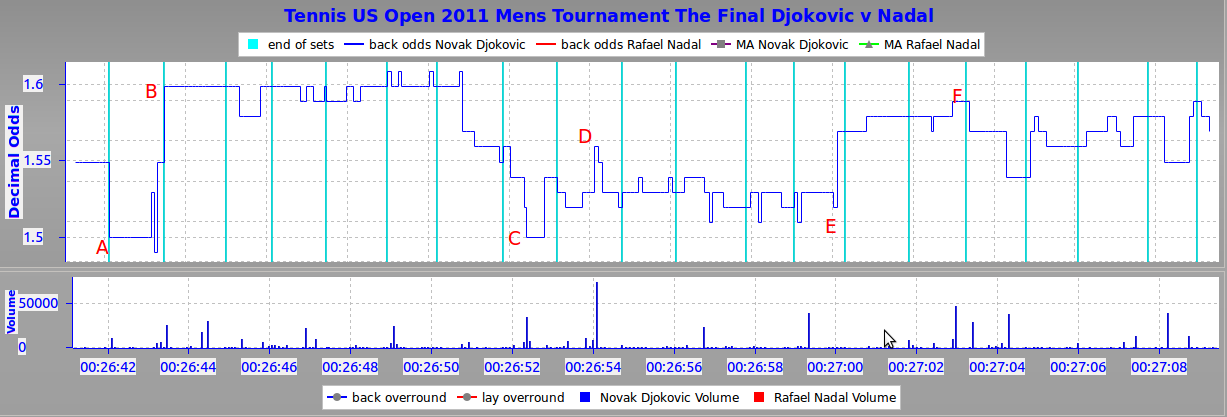
\includegraphics[scale=0.4]{tenistrading.png}
\caption{}
\end{figure}

Now, let's have a look how a professional trader X could make profit from the odds fluctuation during the match.
At point A on the graph, the back odds for N. Djokovic are 1.5. X thinks that the odds are going to grow so he doesn't want to back Djokovic at this point,
instead on the betting exchange he is going to offer to someone else these odds. The offer is accepted by a trader Y who backs Djokovic at 1.5 for a bet of \pounds500. 
At point B, the back odds for N. Djokovic are 1.6. Trader X thinks that the odds are going to fall so he is backing N. Djokovic at 1.6 for a bet of \pounds500. 
He is using the same strategy for points C,D and E,F, so he is offering to someone else odds at points C and E, and is backing at D and F. \\
When the match is over, his bets are as following:\\
Backed N. Djokovic three times at the following odds : 1.6, 1.56,1.58 with a value of each bet of \pounds500. \\
Offered odds to someone else three times at the following values: 1.5,1.5,1.53 with a value of each bet of \pounds500.\\

In case N.Djokovic loses the match, he would lose 3 bets when he backed N. Djokovic but he would win 3 bets because someone else accepted his back odds for N. Djokovic 
and backed N. Djokovic. 
He is losing 3 times \pounds500 but he is winning 3 times back \pounds500, resulting in a P\&L of \pounds0.\\

In case N. Djokovic wins the match, he would win 3 bets when he backed N. Djokovic. \\
His income is going to be: \pounds500 x 1.6+\pounds500 x 1.56+\pounds500 x 1.58 -  \pounds500 x 3 = \pounds870\\
Trader X is going to lose 3 bets because someone else backed N. Djokovic at odds offered by him. \\
His loss is going to be: \pounds500 x 1.5+\pounds500 x 1.5+\pounds500 x 1.53 - \pounds500 x 3  = 765. \\
His final  P\&L in case N. Djokovic wins the match is \pounds870 - \pounds765 = \pounds105

In the tennis trading, professional traders will apply the same strategy as traders in financial markets, Buy Low and Sell High. 

\chapter{User guide}

\section{Installation Instructions}

\section{Quick Start Guide}

\section{FAQ}

\chapter{Exstensive Design}

\chapter{Testing}

\chapter{Statistics}

\chapter{Worklogs}

\end{document}

